%%%%%%%%%%%%%%%%%%%%%%%%%%%%%%%%%%%%%%%%%%%%%%%%%%%%%%%%%%%%%%%%%%%%%%%%%%%%%%%%
%2345678901234567890123456789012345678901234567890123456789012345678901234567890
%        1         2         3         4         5         6         7         8

\documentclass[letterpaper, 10 pt, conference]{ieeeconf}  % Comment this line out
                                                          % if you need a4paper
%\documentclass[a4paper, 10pt, conference]{ieeeconf}      % Use this line for a4
                                                          % paper

\IEEEoverridecommandlockouts                              % This command is only
                                                          % needed if you want to
                                                          % use the \thanks command
\overrideIEEEmargins
% See the \addtolength command later in the file to balance the column lengths
% on the last page of the document

\usepackage[utf8]{inputenc}
\usepackage[T1]{fontenc}
\usepackage{graphicx} %to insert images
% The following packages can be found on http:\\www.ctan.org
%\usepackage{graphics} % for pdf, bitmapped graphics files
%\usepackage{epsfig} % for postscript graphics files
%\usepackage{mathptmx} % assumes new font selection scheme installed
%\usepackage{mathptmx} % assumes new font selection scheme installed
%\usepackage{amsmath} % assumes amsmath package installed
%\usepackage{amssymb}  % assumes amsmath package installed

\title{\LARGE \bf
Matrix Theory Assignment 1
}

%\author{ \parbox{3 in}{\centering Huibert Kwakernaak*
%         \thanks{*Use the $\backslash$thanks command to put information here}\\
%         Faculty of Electrical Engineering, Mathematics and Computer Science\\
%         University of Twente\\
%         7500 AE Enschede, The Netherlands\\
%         {\tt\small h.kwakernaak@autsubmit.com}}
%         \hspace*{ 0.5 in}
%         \parbox{3 in}{ \centering Pradeep Misra**
%         \thanks{**The footnote marks may be inserted manually}\\
%        Department of Electrical Engineering \\
%         Wright State University\\
%         Dayton, OH 45435, USA\\
%         {\tt\small pmisra@cs.wright.edu}}
%}

\author{Ankur Aditya - EE20RESCH11010}



\begin{document}



\maketitle
\thispagestyle{empty}
\pagestyle{empty}


%%%%%%%%%%%%%%%%%%%%%%%%%%%%%%%%%%%%%%%%%%%%%%%%%%%%%%%%%%%%%%%%%%%%%%%%%%%%%%%%
\begin{abstract}

This document contains the procedure to get image of a point in a line. 

\end{abstract}
\\
Download the python code from the below link. Go through the README file in the reposotory.
%
\begin{lstlisting}
https://github.com/ankuraditya13/EE5609-Assignment-1
\end{lstlisting}
%
\\
\begin{comment}
and latex-tikz codes from 
%
\begin{lstlisting}
https://github.com/ankuraditya13/EE5609-Assignment-1
\end{lstlisting}
%
\end{comment}
\section{Problem}

%%%%%%%%%%%%%%%%%%%%%%%%%%%%%%%%%%%%%%%%%%%%%%%%%%%%%%%%%%%%%%%%%%%%%%%%%%%%%%%%
Find the image of the point \left( \begin{array}{c} 3\\ 8\\\end{array}\right) with respect to the line 

   \begin{equation}
         (1\;\;3)\textbf{x} = 7 
\end{equation}       

\section{Solution}


For this problem, I am considering the general case. Let the Equation of line be a*x + b*y = c and let the coordinates of, \\
P(given-point) be \left( \begin{array}{c} x1\\ y1\\\end{array}\right) \\ \\
Q(image-point) be \left( \begin{array}{c} x2\\ y2\\\end{array}\right) \\ \\
R(point-on-mirror) be \left( \begin{array}{c} x3\\ y3\\\end{array}\right) \\
\\

Let vector n = \left( \begin{array}{c} a\\ b\\\end{array}\right)
\\ \\
\textbf{Let m be the directional vector along line a*x + b*y = c.}\\ \textbf{ Hence, m = (b -a) } \\ 

Let m1 and m2 be the slopes of two prependicular lines,\\ \\
Now, m1 = \(\frac{y2 - y1}{x2 - x1}\) and m2 = \(\frac{-a}{b}\)\\     \\ 
Now for perpendicular lines m1 * m2 = -1, which in vector can be written as:\\
\begin{equation}
   m^T * R = m^T * P;  
\end{equation}

Similarly in vector form line equation a*x + b*y + c = 0 is given as,
\begin{equation}
    n^T * Q = c;
\end{equation}


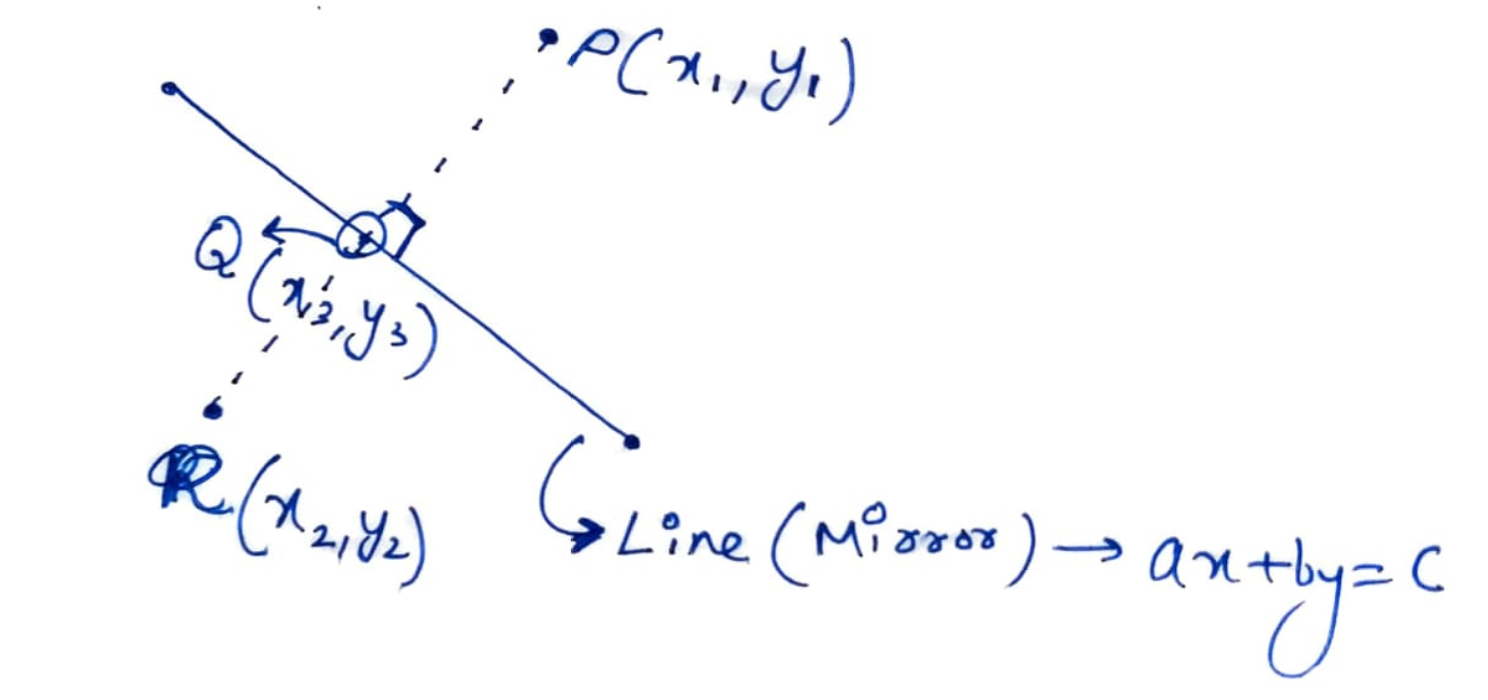
\includegraphics[scale=0.25]{fig1.png} \\


By property in Figure 1, the line PR bisects the mirror equation perpendicularly. Hence, 
\begin{equation}
    2*Q = P + R
\end{equation}

Hence, From the equation (3) and (4)
\begin{equation}
    n^T * R = 2*c - n^T * P
\end{equation}
Now, form equation (5) and (2) we get,

\begin{equation}
    (m\hspace{0.5cm}n) ^T * R = (m\hspace{0.35cm}-n) ^T * P + (0\hspace{0.35cm}2*c) ^T
\end{equation}
Hence upon solving the equation for point R using the property,
(m\hspace{0.35cm}-n) = (m\hspace{0.5cm}n) * \left( \begin{array}{c} 1\hspace{0.25cm}0\\  0\hspace{0.1cm}-1\\\end{array}\right) \textbf{we get,} \\ 

\\
\begin{equation}
    \(\frac{R}{2}\) = \(\frac{m * m^T - n*n^T}{m^T * m + n^T * n}\) *P + c * \(\frac{n}{||n||^2}\)
\end{equation}


     
 Hence, substituting the value of x1 = 3, y1 = 8, a = 1, b = 3 and c = 7 we get,\\ \\
 P(given-point)  = \left( \begin{array}{c} 3\\ 8\\\end{array}\right) \\ \\
 m(direction-vector) = \left( \begin{array}{c} 3\\ -1\\\end{array}\right) \\ \\
 n = \left( \begin{array}{c} 1\\ 3\\\end{array}\right) \\ \\
 Norm, ||n|| = (a^2+b^2)^(0.5) \\  \\
 
\textbf{ Substituting these values in equation (7) we get,\\ \\
 R = \left( \begin{array}{c} -1\\ -4\\\end{array}\right) \\ \\
 \textbf{Hence, it is the required answer for image of P in line \\(1 3) x =7.} }
 











\end{document}
